\documentclass[a4paper,11pt,twoside]{scrartcl}
\usepackage[T1]{fontenc}
\usepackage{subcaption}
\usepackage[utf8]{inputenc}
\usepackage{ngerman, eucal, mathrsfs, amsfonts, bbm, amsmath, amssymb, stmaryrd,graphicx, array, geometry, color, wrapfig, float, hyperref, epstopdf,gensymb, subcaption, extarrows}
\usepackage[controls, step, poster=first]{animate}
\geometry{left=25mm, right=15mm, bottom=25mm}
\setlength{\parindent}{0em} 
\setlength{\headheight}{0em} 
\title{Graphenalgorithmen\\ Blatt 10}
\author{Markus Vieth\and Christian Stricker}
\date{\today}
\input{../head/lstlisting.tex}
\usepackage{float}
\usepackage[section]{placeins}
\usepackage{epstopdf}
\usepackage{wrapfig}
\usepackage{caption}
\usepackage{subcaption}
\usepackage{graphicx}
\usepackage{pgfplots}
\usepackage[usenames,dvipsnames,svgnames,table]{xcolor}
\usetikzlibrary{plotmarks}
\usetikzlibrary{patterns}
\usetikzlibrary{decorations.pathmorphing}
\usetikzlibrary{calc}
\usetikzlibrary{shapes}
\newcommand{\coloredcircled}[3][black]{{\large \Large\color{#2}\textcircled {{\small\color{#1}#3}}}}% Circlecolor, Textcolor, text
\newcommand{\ddvec}[2]{\begin{pmatrix}#1\\#2\end{pmatrix}}
\newcommand{\dddvec}[3]{\begin{pmatrix}#1\\#2\\#3\end{pmatrix}}
\newcommand{\longvec}[1]{\overset{\longrightarrow}{#1}}
\newcommand{\eunorm}[1]{\left\lVert#1\right\rVert_2}
\newcommand{\scalar}[2]{\left<#1,#2\right>}\newcommand{\cor}[1]{\textcolor{red}{\textit{#1}}}
\newcommand{\qed}{%
	\begin{flushright}
		q.e.d.
	\end{flushright}%
	}
\begin{document}
\maketitle
\cleardoublepage
\pagestyle{myheadings}
\markboth{Markus Vieth, Christian Stricker}{Markus Vieth, Christian Stricker}

\newpage
\section{Aufgabe 1: Weighted-Circuit-Satisfiability(WCS) (5+5=10 Punkte)}
\begin{figure}[H]
	\centering
	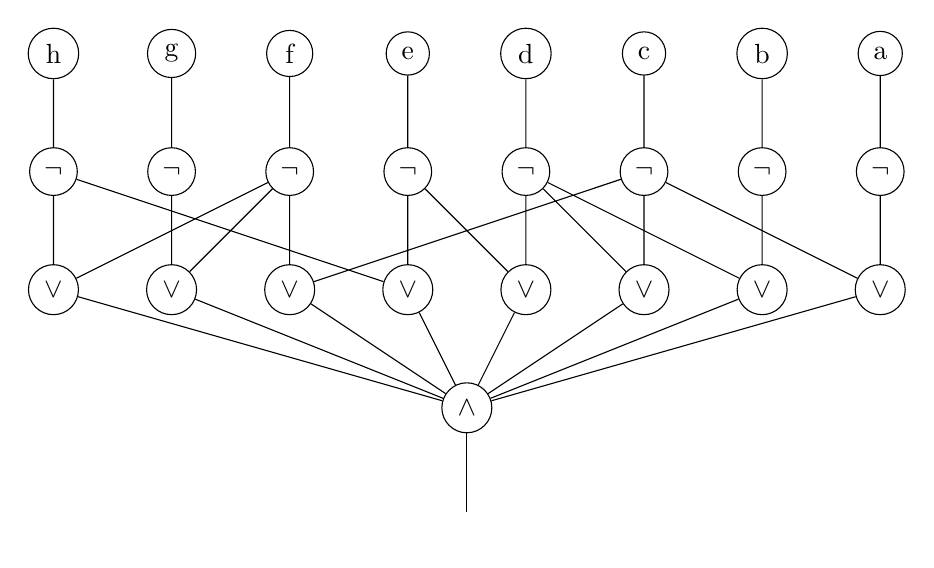
\begin{tikzpicture}[every node/.style = {draw, align=center, circle}, rotate = 180]
	\node[draw = white] {}
	child {
		node {$\land$}
		child {
			node (ac){$\lor$}
			child {
				node (a){$\neg$}
				child {node {a}}	
			}
		}
		child {
			node (bd){$\lor$}
			child {
				node (b){$\neg$}
				child{node {b}}	
			}
		}
		child {
			node (cd) {$\lor$}
			child {
				node (c) {$\neg$}
				child{node{c}}	
			}	
		}
		child {
			node (de) {$\lor$}
			child {
				node(d){$\neg$}
				child{node{d}}
			}	
		}
		child {
			node (eh) {$\lor$}
			child {
				node(e){$\neg$}
				child{node{e}}	
			}	
		}
		child{
			node (cf) {$\lor$}
			child {
				node (f) {$\neg$}
				child{node{f}}	
			}	
		}
		child {
			node (fg) {$\lor$}
			child {
				node(g) {$\neg$}
				child{node{g}}	
			}
		}
		child {
			node (fh) {$\lor$}
			child {
				node(h) {$\neg$}
				child{node{h}}
			}	
		}
	};
	\draw (c) -- (ac) (d)--(bd) (d) -- (cd) (e)--(de) (h)--(eh) (c)--(cf) (f)--(fg) (f)--(fh);
	\end{tikzpicture}
	\caption{a}
\end{figure}
\begin{figure}[H]
	\centering
		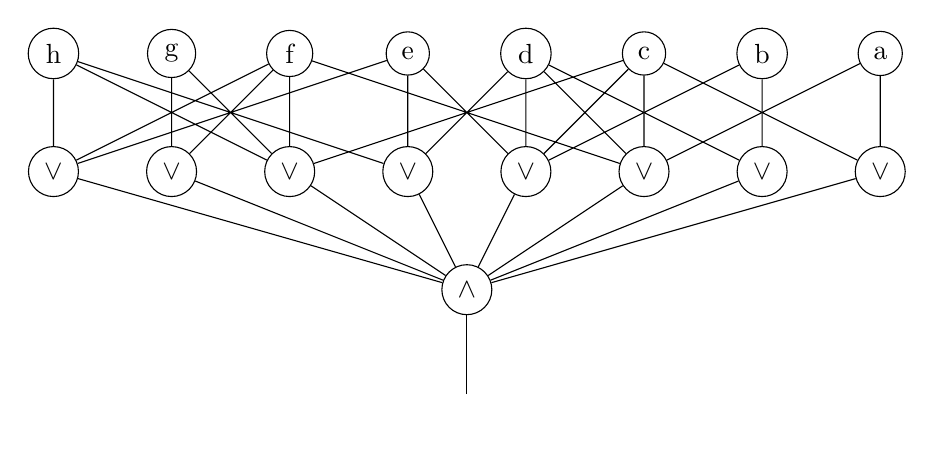
\begin{tikzpicture}[every node/.style = {draw, align=center, circle}, rotate = 180]
			\node[draw = white] {}
				child {
					node {$\land$}
					child {
						node (A) {$\lor$}
							child {
								node (a){a}	
							}
					}
					child {
						node (B){$\lor$}
						child {
							node (b) {b}	
						}
						}
						child {
							node (C){$\lor$}
							child {
								node (c){c}	
							}
						}
						child {
							node (D){$\lor$}
							child {
								node (d){d}	
							}
						}
						child {
							node (E){$\lor$}
							child {
								node (e){e}	
							}
						}
						child {
							node (F){$\lor$}
							child {
								node (f){f}	
							}
						}
						child {
							node (G){$\lor$}
							child {
								node (g){g}	
							}
						}
						child {
							node (H){$\lor$}
							child {
								node (h){h}	
							}
						}
				};
			\draw (c) -- (A) (d) -- (B) (a)--(C) (f)--(C) (d)--(C) (c)--(D) (e)--(D) (b)--(D) (d)--(E)	(h)--(E) (c)--(F) (h)--(F) (g)--(F) (f)--(G) (f)--(H) (e)--(H);
			
		\end{tikzpicture}
		\caption{b}
\end{figure}
\section{Aufgabe 2: Parametrisierte-Reduktion (10 Punkte)}
Es sei als Eingabe:$\text{WCS}[C_{t,ds}]$
\begin{align*}
C&=\{S_1,\ldots,S_n \}&\text{ with }&X = \bigcup_{S\in C}S=\{ x_1,\ldots,x_m \}
\end{align*}
Ich definiere den Graphen:
\[ G=(V,E) \]
\[ V = \{ 1,2,\ldots,n,x_1,x_2,\ldots,x_m \} \]
\[ E = \{ (i,j): 1 \leq i < j \leq n \} \cup \{ (i,x) : 1 \leq i \leq n \land x \in S_i \} \]
Somit sind die Knoten 1 bis $n$ vollständig verbunden, während die Knoten $x_1$ bis $x_m$ nicht untereinander verbunden sind.\\
Ein gegebenes dominating set $W \subseteq V$ von $G$ kann nun wie folgt in ein Set Cover umgewandelt werden:\\
\begin{enumerate}
	\item Nimm einen Knoten $x_i \in W$
	\item Ersetzte in mit einem Knoten $v \in \{i:(i,x_j)\in E\}$ (wir erhalten weiterhin ein dominating set identischer Größe)
	\item Wiederhole Schritte 1 und 2 bis kein $x_j$ mehr in $W$ vorhanden ist.
	\item Konstruiere eine Lösungsmenge für $X$ mit $\{ S_i\in C : i \in W \}$. Offensichtlich hat dieses Set die Größe $|W|$
\end{enumerate}
Wir können für jedes Set Cover $C' \subseteq C$ ein dominating set $W\subseteq V$ der selben Größe konstruieren, indem wir die Knotenmenge $\{ i : S_i \in C' \}$ hinzufügen.
\section{Aufgabe 3: WCS -Definition (10+10=20 Punkte)}
\subsection{a}
Große Knoten lassen sich auf kosten der Baumtiefe in kleine Knoten aufteilen. Dabei steigt die Baumtiefe logarithmisch.
\subsection{b}
Aus der Teilaufgabe a folgt:\\
Für $t,d \geq 1, s\geq 2$ existiert eine parametrisierte Reduktion von $\text{WCS}[C_{s,t,d}]$ auf $\text{WCS}[C_{t,ds}]$. Somit folgt, dass ein Problem, dass auf $\text{WCS}[C_{s,t,d}]$ parametisiert reduzierbar ist für ein festes $s$ auch auf  $\text{WCS}[C_{t,ds}]$ reduzierbar ist. Somit gilt die Behauptung.
\end{document}